\documentclass[11pt,letterpaper]{article}
\usepackage{naaclhlt2015}
\usepackage{times}
\usepackage{latexsym}
\usepackage{url}
\usepackage[pdftex]{graphicx}
\usepackage{breqn}
\usepackage{multirow}
\setlength\titlebox{6.5cm}    % Expanding the titlebox

%%%%%%%%%%%%%%%%%%%%%%%%%%%%%%%%%%%%%%%%%%%%%%%%%%%%%%%%%%%%%%%%%%%%%%
% Code to use with NAACL/ACL style files to simulate natbib's 
% \citealt, which prints citations with no parentheses. This should
% work if pasted into the preamble. \cite, \newcite, and \shortcite
% should continue to work as before.

\makeatletter

\def\citealt{\def\citename##1{{\frenchspacing##1} }\@internalcitec}

\def\@citexc[#1]#2{\if@filesw\immediate\write\@auxout{\string\citation{#2}}\fi
  \def\@citea{}\@citealt{\@for\@citeb:=#2\do
    {\@citea\def\@citea{;\penalty\@m\ }\@ifundefined
       {b@\@citeb}{{\bf ?}\@warning
       {Citation `\@citeb' on page \thepage \space undefined}}%
{\csname b@\@citeb\endcsname}}}{#1}}

\def\@internalcitec{\@ifnextchar [{\@tempswatrue\@citexc}{\@tempswafalse\@citexc[]}}

\def\@citealt#1#2{{#1\if@tempswa, #2\fi}}

\makeatother
%%%%%%%%%%%%%%%%%%%%%%%%%%%%%%%%%%%%%%%%%%%%%%%%%%%%%%%%%%%%%%%%%%%%%%

% Effects of non-linguistic context
\title{Audience size and noise levels modulate information density in Twitter conversations}
% Information content changes with audience and conversation length in microblog texts
% common ground decreases information

\author{Gabriel Doyle\\
Dept. of Psychology\\
Stanford University\\
Stanford, CA, USA, 94305\\
{\tt gdoyle@stanford.edu}
	  \And
          Michael C. Frank\\
Dept. of Psychology\\
Stanford University\\
Stanford, CA, USA, 94305\\
{\tt mcfrank@stanford.edu}
}

\date{}


\begin{document}
\maketitle
\begin{abstract}
Optimal use of a noisy communication channel requires the uniform distribution of information across a message; the ``uniform information density'' (UID) hypothesis proposes that language producers aim for such uniformity. Previous research on monologue-like written texts has suggested that discourse context induces adaptations in production to maintain UID.  We consider conversational messages, using a large corpus of tweets, and look for UID behavior in interactive conversation.  We do not find evidence of UID behaviors, and even find context effects that are opposite that of previous, monologue-based research.  We propose possible explanations for these findings within an information-theoretic framework.

\end{abstract}

\section{Introduction}

Linguistic communication can be viewed from an information theoretic standpoint as communication via a noisy channel.  If humans are approximately rational in their communications and the noisy channel model is appropriate, then we expect to see communication follow an approximately constant rate of information flow.  This is the Uniform Information Density (UID) hypothesis.

Evidence in favor of UID has been found in many levels of language production. At the level of within-sentence context, there is clear evidence from phonology that speakers reduce more predictable sounds \cite{aylett2004,aylett2006,bell2003,demberg2012}, suggesting that they are giving more ``air time'' to less predictable material to equalize information density. And in syntax, speakers tend to drop optional materials (like the word ``that'' as a sentence-complementizer) in more predictable scenarios \cite{levy2007,frank2008,jaeger2010}, again implying a process of allocating communication time relative to predictability. These effects appear in both monologues and dialogues, suggesting that local linguistic context shapes message complexity.

There is also some evidence for UID based on broader, discourse-level context.  \citealt{genzel2002} showed that word-by-word complexity (measured by a standard n-gram language model) increases across sequences of sentences. They hypothesized that this increase was due to a corresponding increase in non-linguistic information that would make even more complex linguistic structures easier to predict. Follow-ups have shown that this same complexity increase effect is attested in different document types and across languages \cite{genzel2003,qian2012}. However, these studies draw almost exclusively from long, well-structured written texts that function as monologues from writer to reader.  

This leaves an important gap in these tests of the UID hypothesis: little work has looked at the influence of discourse-level context on information structure in interpersonal dialogue, the archetype of human linguistic communication.  With the exception of one preliminary study that provided a partial replication of the original complexity increase effect using the Switchboard corpus \cite{vega2009}, to our knowledge no work has explored how the broader dynamics of conversation interact with UID. 

The present study applies information-theoretic analysis to a corpus of social media microblog posts that include a large number of natural dialogues.  Surprisingly, we do not see clear evidence of the UID hypothesis in these dialogues.  Instead, we propose that differences in the discourse-level structure of conversation compared to monologues may interfere with attaining UID in the standard formulation.

\subsection{Conversations, context, and content}

One common motivation for the UID hypothesis is a rational analysis based on a noisy-channel model of communication \cite{levy2007}.\footnote{The other common motivation is a surprisal-based argument \cite{levy2008}: maintaining UID also minimizes the listener's comprehension effort.}  In the noisy-channel analysis, the amount of noise in the channel sets an optimal value for information density to obtain fast, error-free transmission.  For a noise level $\alpha$, we will refer to the optimal information content per discourse unit $Y_i$ as $H_\alpha(Y_i)$.  Discourse units, depending on the analysis, range from syllables to whole documents; in our analyses, we focus on words and tweets as our discourse units.

In the course of a message, as argued by \newcite{genzel2002}, the actual information content per discourse unit is predicted by the entropy of the random variable $X_i$ representing the precise word choice or choices within the discourse unit, conditioned on the available context.  The precise extent of this context is difficult to pin down. 

We estimate context for our dialogue studies by thinking in terms of the {\it common ground} that a rational speaker believes to exist, given the expected audience of their message. Common ground is defined as the knowledge that participants in a discourse have and that participants know other participants have, including the current conversational context \cite{clark1996}. This common ground can be built from a combination of linguistic and non-linguistic context, including previous messages within the discourse, preceding interactions between the conversation participants, and world knowledge. %about the topic being discussed.

To formalize this relationship, let $C_i$ be the common ground that exists prior to the production of discourse unit $Y_i$, and let $\alpha$ be the expected noise level in the channel that $Y_i$ is transmitted through.  Then optimality within a noisy channel model predicts that the noise-dependent optimal information rate $H_{\alpha}(Y_i)$ is related to the actual information rate as follows:

\begin{equation}
H_{\alpha}(Y_i|C_i) =  H(X_i) - I(X_i ; C_i) \label{eq:uid}
\end{equation}

Here, $H(X_i)$ is the apparent decontextualized entropy of the discourse unit independent of the common ground.  This quantity is often estimated from a language model that uses only local context, not higher-level discourse context or common ground.  We use a trigram Markov model in this study.

$I(X_i;C_i)$ is the mutual information of the discourse unit random variable $X_i$ and the common ground $C_i$---essentially how much more predictable the next discourse unit becomes from knowing the common ground.  Common ground is difficult to quantify---both in the particular datasets we consider and more generally---so we rely on the assumption that more common ground is correlated with greater mutual information, as in \newcite{genzel2002}.

Then, based on this assumption, Eq. \ref{eq:uid} allows us to make two UID-based predictions. First, as channel noise increases, transmission error should increase, which in turn should cause the optimal information transfer rate $H_\alpha(Y_i)$ to decrease.  Thus, to maintain equality with rising noise, the apparent entropy $H(X_i)$ should decrease. This prediction translates into communicators ``slowing down'' their speech (albeit in terms of information per word, rather than per unit time) to account for increased errors. 

Second, as common ground increases, $I(X_i;C_i)$ should increase. To maintain equality with rising common ground, $H(X_i)$ should thus also increase, so as not to convey information slower than necessary. This prediction translates into communicators ``going faster'' (e.g., packing more information into each word) because of an assumption that listeners share more common ground with them.

\subsection{The current study}

We take advantage of the conversational structure of the popular social media microblogging platform Twitter (\url{http://twitter.com}) to test these predictions.  Twitter allows users to post 140 character ``tweets'' in a number of different conversational contexts. In particular,  because some tweets are replies to previous tweets, we can use this reply structure to build conversational trees, and to track the number of participants.  In addition, specific choices in tweet production can affect what audience is likely to see the tweet.  These variables are discussed in depth in Section \ref{sect:conversation}.

To test the entropy effects predicted by Eq. \ref{eq:uid}, we first examine different types of tweets that reach different audience sizes.  We then restrict our analysis to reply tweets with varying audience sizes to analyze audience size independently of noise.  Finally, we look at the effects of common ground (by way of conversation structure) on tweet entropy. Contrary to previous UID findings, we do not see a clear increase in apparent entropy estimates due to more extensive common ground, as had been found in previous non-conversational work \cite{genzel2002,qian2012,doyle2015}.  

We propose two factors that may be influencing conversational content in addition to UID factors.  First, achieving conversational goals may be more dependent on certain discourse units that carry low linguistic informativity but substantial social/conversational importance.  Second, considering and adapting to two different types of noise---message loss and message corruption---may cause tweeters to make large-scale decisions that overwhelm UID effects.

\section{Corpus}

Randomly sampling conversations on a medium like Twitter is a difficult problem. Twitter users routinely use the medium to converse in smaller groups via the \@ mention functionality (described in more detail below). Yet such conversations are not uniformly distributed: A random sample of tweets---perhaps chosen because they contain the word ``the'' or a similarly common token \cite{doyle2014}---yields mostly isolated tweets rather than complete dialogues. Dialogues depend on users interacting back and forth within communities.  %Dialogues tend to occur because a user with a sufficient community of followers posts a tweet that causes followers to engage and then responds to at least some of the followers' reactions. 

\subsection{Seed strategy}

To sample such interactions, we developed a ``seed'' strategy where we identified popular Twitter accounts and then downloaded a large sample of their tweets, then downloaded a sample of the tweets of all the users they mentioned. This strategy allowed us to reconstruct a relatively dense sample of dialogues (reply chains).

\begin{table}
\begin{center}
\begin{tabular}{|c|c|c|c|}
\hline
Seed Users & Category \\ % & Replies & Non-replies\\
\hline
{\tt @camerondallas} & \multirow{2}{*}{Youtube stars} \\
{\tt @rickypdillon} & \\
\hline
{\tt @edsheeran} & \multirow{2}{*}{Musicians} \\
{\tt @yelyahwilliams} & \\
\hline
{\tt @felixsalmon} & \multirow{2}{*}{Journalists} \\
{\tt @tanehisicoates} & \\
\hline
{\tt @jahimes} & \multirow{3}{*}{Politicians} \\
{\tt @jaredpolis} & \\
{\tt @leezeldin} & \\
\hline
{\tt @larrymishel} & \multirow{2}{*}{Economists} \\
{\tt @paulnvandewater} & \\
\hline
{\tt @neiltyson} & \multirow{3}{*}{Scientists} \\
{\tt @profbriancox} & \\
{\tt @richardwiseman} & \\
\hline
\end{tabular}
\end{center}
\caption{\label{tab:seed-users} Seed users for our dataset.}
\end{table}

We began by choosing a set of 14 seed Twitter accounts (Table \ref{tab:seed-users}) that spanned a variety of genres, were popular enough to elicit replies, and interacted with other users often enough to build up a community. 

To build conversations, we needed to obtain tweets directed to and from these seed users. For each seed user, we downloaded their last 1500 tweets, extracted all users mentioned within those tweets, and downloaded each of their last 1500 tweets.  To capture tweets that failed to start conversations with the seed users, we also added the last 1000 tweets mentioning each seed user's handle.  Tweets that appeared in multiple communities were removed.  Each reply contains the ID of the tweet it replies to, so we could rebuild conversation trees back to their roots, so long as all of the preceding tweets were made by users in our communities.

\subsection{Conversation structure and visibility}\label{sect:conversation}

Twitter conversations follow a basic tree structure with a unique root node. Each tweet is marked as a reply or not; for replies, the user and tweet IDs of the tweet it replies to is stored. Each tweet can be a reply to at most one other tweet, so a long conversation resembles a linked list with a unique root node. ``Mentions,'' the inclusion of a username in a tweet, are included in tweets by default throughout a conversation unless a tweeter chooses to remove some of them, so tweets deep in a conversation may be primarily composed of mentions rather than new information.  

%Mentions also affect tweet visibility.  Tweets whose first character is a mention (whether or not it is a reply) do not show up by default when browsing a user's tweets, unless the browser follows both the tweeter and first-mentioned user.\footnote{This behavior varies slightly depending on what application is used to view Twitter.  On the website, mention-first tweets do not appear in lists and only appear after clicking the 'tweets \& replies' option on a timeline. On the Twitter mobile app, mention-first tweets appear by default on a timeline but still not in lists.}

After some processing described below, our sampling process resulted in 5.5 million tweets, of which 3.3 million were not part of a conversation (not a reply, and received no replies).  Within this data, we found 63,673 conversations that could be traced back to a root tweet, spanning 228,923 total tweets. Unfortunately, Twitter only tracks replies up a tree, so while we know with certainty whether a tweet is a reply (even if it is to a user outside our communities), we do not know with certainty that a tweet has received no replies, especially from users outside our communities. If anything, this fact makes our analyses conservative, as they may understate differences between reply and non-reply tweets. The remaining 2 million tweets were replies whose conversations could not be traced back to the root.

\subsection{Information content estimation}

To estimate the information content of a tweet, we first tokenized the tweets using Twokenizer \cite{owoputi2013}. We then removed any number of mentions at the beginning or end of a tweet, as these are usually used to address certain users rather than to convey information themselves. (Tweets that only contained mentions were removed.)  Tweet-medial mentions were retained but masked with the single type {\it [MENTION]} to reduce sparsity. Links were similarly masked as {\it [URL]}. Punctuation and emoji were retained. We then built trigram language models using SRILM with default settings and Kneser-Ney discounting.  Types with fewer than 5 tokens were treated as out-of-vocabulary items. 

For each community, the training set was the set of all tweets from all other communities.  This training set provides tweets that are contemporaneous to the test set and cover some of the same topics without containing the same users' tweets.

\section{Analyses}

We describe the results of three sets of analyses looking at the influence of audience size and available context on apparent tweet entropy. The first examines the effect of expected audience size at a coarse level, comparing tweets directed at a small subset of users, all one's followers, or the wider realm of a hashtag.   The second examines the effect of finer differences in known audience size on apparent informativity.  The third examines the effects of conversational context and length on informativity.

\subsection{Expected audience size}
\label{sec:expected}

First, we consider three different types of tweets and their expected audience size.  Tweets whose first character is a mention (whether or not it is a reply) do not show up by default when browsing a user's tweets, unless the browser follows both the tweeter and first-mentioned user.\footnote{This behavior varies slightly depending on what application is used to view Twitter.  On the website, mention-first tweets do not appear in lists and only appear after clicking the 'tweets \& replies' option on a timeline. On the Twitter mobile app, mention-first tweets appear by default on a timeline but still not in lists.} We will refer to these as ``invisible'' tweets as they are invisible to followers by default.  A tweeter making an initial-mention tweet thus should expect such a tweet to have a relatively limited audience, with a focus on the mentioned users.\footnote{Some Twitter users consciously manipulate audience using these markers: many tweets have an initial period or other punctuation mark to prevent it from being hidden. Some users routinely switch between initial-mention replies and ``dot''-replies in the course of a conversation to change the audience, presumably depending on their estimate of the wider relevance of a remark.}

\begin{table*}
  \begin{tabular}{|c|l|c|}
\hline
Type & Tweet & Per-word entropy \\
\hline
\multirow{3}{*}{invisible\vspace*{-.7em}} & [MENTION] [MENTION] this is so accurate tho & 6.00\\
\cline{2-3}
 & [MENTION] can you come to my high school ? ;3 & 7.61\\
\cline{2-3}
 & \parbox[][6ex][c]{.7\textwidth}{[MENTION] Hi Kerry , Please send us your email address in order to discuss this matter further . Thanks !} & 8.58\\
\hline
\hline
 & post your best puns in the comments of my latest instagram photo : [URL] & 7.44\\
\cline{2-3}
\multirow{2}{*}{baseline}  & \parbox[][6ex][c]{.7\textwidth}{ I wish I could start a blog dedicated to overly broad and sweeping introductory sentences} & 9.98\\
\cline{2-3}
&\parbox[][6ex][c]{.7\textwidth}{ this new year's eve in NYC , keep an eye peeled 4 Sad Michael Stipe . [URL] already found him : [URL]} & 7.17\\
\hline
\hline
 & I will probably be quitting my job when \#GTAV comes out & 7.63\\
\cline{2-3}
\multirow{2}{*}{hashtagged} & \parbox[][6ex][c]{.7\textwidth}{\#UMAlumni what is the number one thing graduating seniors should know ? \#MGoGrad} & 6.80\\
\cline{2-3}
 & \parbox[][6ex][c]{.7\textwidth}{Brilliant interactive infographic : shows cone of uncertainty for \#climatechange [URL] \#howhotwillitget} & 12.1\\
\hline
  \end{tabular}
 \caption{Example tweets from each category.}\label{tab:ex}\vspace*{-.5em}
\end{table*}


On the other side, a hashtag serves as a categorization mechanism so that interested users can discover new content. Hashtags are often used to expand the potential audience for a tweet to include the feeds of users tracking that hashtag, regardless of whether they follow the original tweeter, and so a tweeter using a hashtag should expect a larger audience than normal.\footnote{Not all hashtags are intended for categorization; some are used for emphasis or metalinguistic comment (e.g. \#notmyfavoritefridaymeal, \#toomuchinformation). These comments are probably not intended to broaden the tweet's audience. The presence of such hashtags should, if anything, cause our analysis to underestimate variability across audience types.}  Finally, we have baseline tweets which contain neither mentions nor hashtags and whose expected audience size is approximately one's followers.

Intuitively, common ground is higher for smaller audiences. It should be highest for the invisible tweets, where the audience is limited and has seen or can readily access the previous tweets in the conversation.  It should be lowest for the hashtagged tweets, where the audience is the largest and will likely contain many users who are completely unfamiliar with the tweeter.  If contextualized UID is the driving force affecting information content, then the invisible tweets should have the highest entropy and hashtagged tweets should have the lowest.

\begin{figure}
 \centering 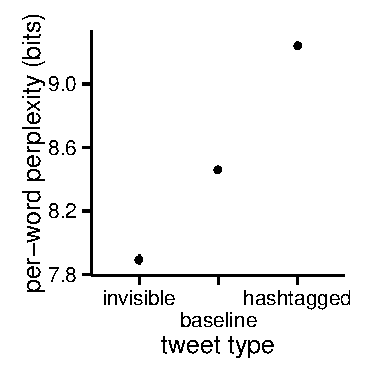
\includegraphics[width=1.7in]{figures/cmcl-audience-pw.pdf}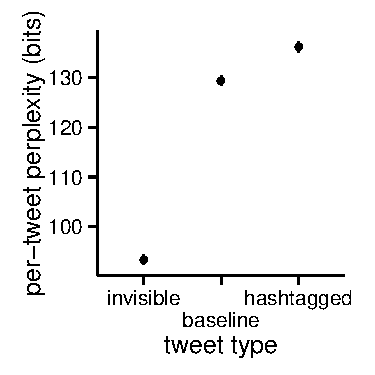
\includegraphics[width=1.7in]{figures/cmcl-audience-pt.pdf}
 \caption{\label{fig:audience} Per-word (left) and per-tweet (right) entropy are higher for tweets with larger expected audience size. By-user 95\% confidence intervals.}
\vspace*{-.5em}
\end{figure}

In this analysis, we use the full 5.5 million tweet database. Figure \ref{fig:audience} plots the entropy of tweets for these three audience sizes.  Per-word and per-tweet entropy both significantly {\it increase} with expected audience size ($p < .001$ by likelihood-ratio test), the opposite direction of our prediction. We discuss this finding below in the context of our next analyses. 


\subsection{Known audience size}

The results from expected audience size in Section \ref{sec:expected} have a potential explanation: different tweet types are received and viewed in different ways, which may encourage different kinds of communicative behavior.  Tweets with mentions are highly likely to be seen by the mentioned user (unless the mentioned user is very popular), whereas the likelihood of a given hashtagged tweet being seen through the hashtag-searching mechanism is very low.  This uncertainty about audience may lead a rational tweeter to package information into tweets differently: they may include more redundant information across tweets when the likelihood of any given tweet being read is low.

To assess audience size effects in a more controlled setting, we look at invisible tweets with varying numbers of mentions.  Invisible tweets provide a quantifiable audience size; those with few mentions have a smaller audience than those with more mentions.  Visible tweets, on the other hand, have approximately the same audience size regardless of the number of mentions, since all of a user's followers can see them. Visible mentions can be used for a wide range of discourse functions (e.g., self-promotion, bringing one's followers into an argument, entering contests), and so we do not have a clear prediction of their behavior. But invisible mentions should, under the UID hypothesis, show decreased common ground as the number of conversation participants grows and it is harder to acheive consensus on what all participants know.

\begin{figure}[t]
 \centering
  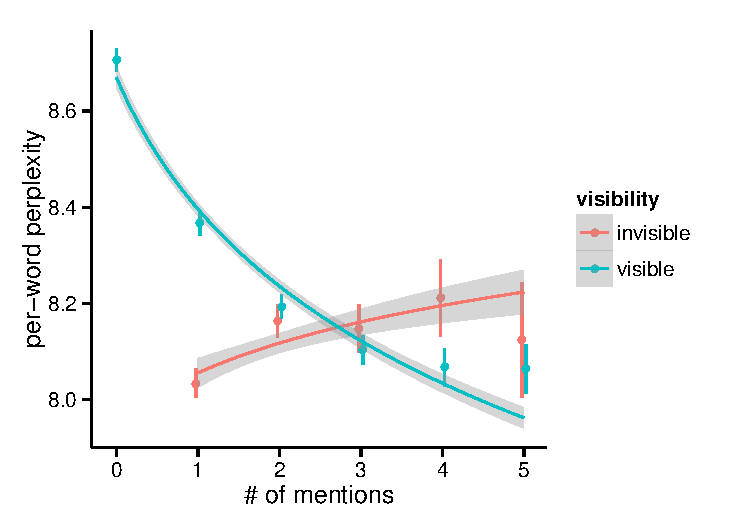
\includegraphics[width=3.25in]{figures/cmcl-mentions-pw2.pdf}
  % 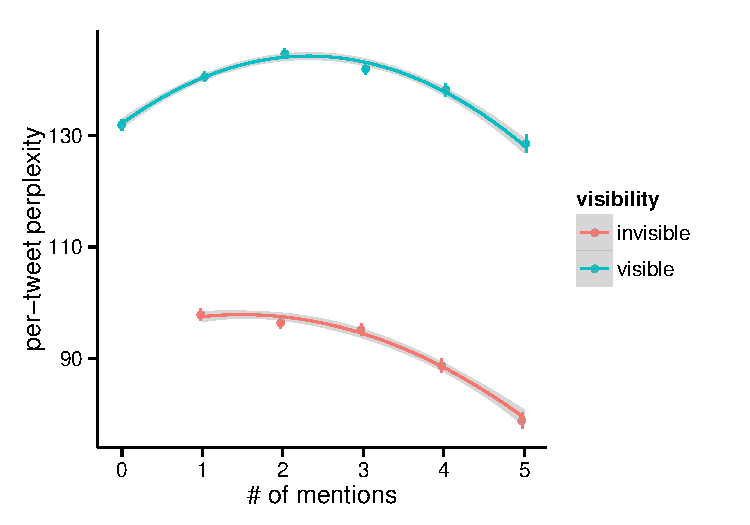
\includegraphics[width=3.25in]{figures/cmcl-mentions-pt.pdf}
 \caption{Per-word entropy of tweets with different numbers of mentions and different visibility.  Invisible tweets' entropy increases with mentions, while visible tweets' entropy decreases. Logarithmic fits with 95\% confidence intervals; x-axis is log-scaled.}\label{fig:mentions}\vspace*{-.5em}
\end{figure}

Figure \ref{fig:mentions} shows that the per-word entropy of invisible tweets goes up with the logarithm of the number of mentions.   We look only at tweets with between one and five mentions, as invisible tweets must have at least one mention, and five mentions already substantially cut into the 140-character limit.\footnote{Usernames can be up to 15 characters (plus a space and an \@ symbol per mention); even if each username is only 7 characters, five mentions use almost one-third of the character limit.}  This leaves 1.4 million tweets.

The fact that invisible tweet entropy increases with number of mentions, even as visible tweet entropy decreases, suggests that audience size is having an effect.  However, this effect is causing entropy to increase as common ground should be decreasing due to the larger number of conversation participants.  Furthermore, this effect is not driven by reply level (Sect \ref{sect:reply-level}); there is a significant increase ($p < .001$) in explanatory power from adding number of mentions to a mixed-effects model with fixed-effects of reply level and a by-user random intercept.

\subsection{Reply level and conversation length}\label{sect:reply-level}

\begin{figure}[t]
 \centering
  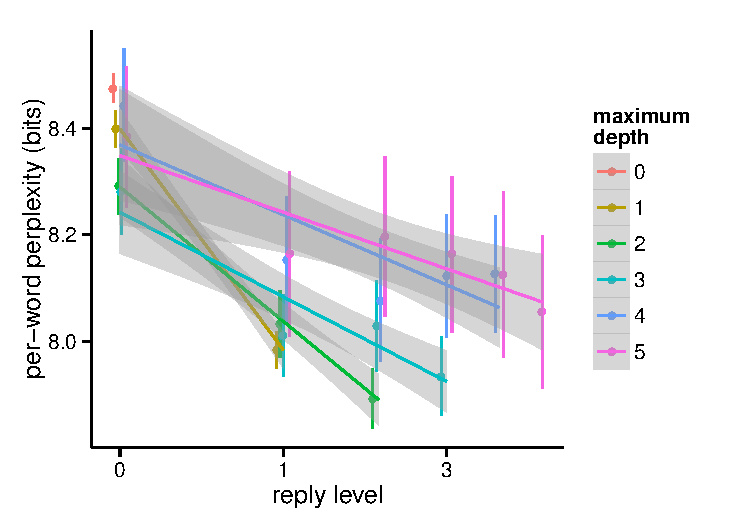
\includegraphics[width=3.25in]{figures/cmcl-rlevel-pw.pdf}\vspace*{-.3em}
  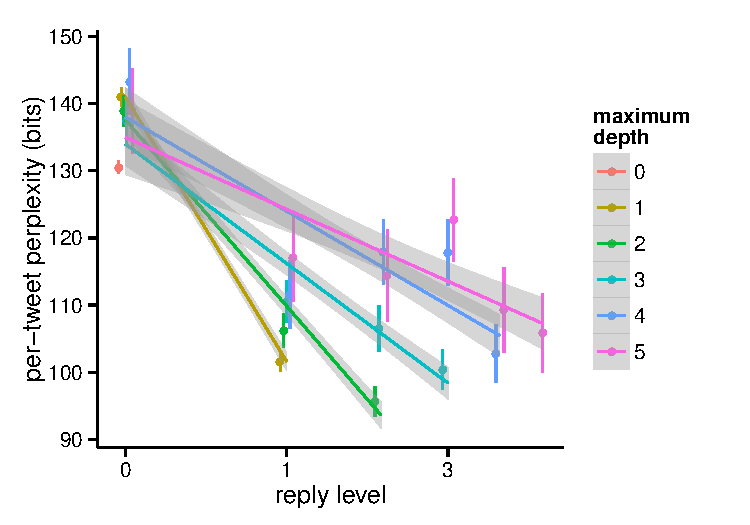
\includegraphics[width=3.25in]{figures/cmcl-rlevel-pt.pdf}\vspace*{-.3em}
 \caption{Per-word (top) and per-tweet (bottom) entropy decrease with reply level and increase with conversation length.  Logarithmic fits with 95\% confidence intervals; x-axis is log-scaled.}\label{fig:rlevel-maxdesc}\vspace*{-.5em}
\end{figure}

We next turn to our second UID prediction: that information content should increase as common ground increases. As common ground is assumed to increase in dialogues \cite{clark1996}, we thus predict that Twitter conversations should show increases in information content that scale with reply level, the number of replies between the current tweet and the conversation root. Such a result would constitute a replication of \citealt{genzel2002} in the discourse context, and would confirm preliminary results on the Switchboard corpus by \citealt{vega2009}. As is clear from our analysis below, that is not what we found. 
	
Figure \ref{fig:rlevel-maxdesc} plots mean perplexities for different reply levels and conversation lengths, with confidence intervals based on by-user means. Increasing the reply level decreases the information content of the tweet, while increasing the conversation length increases the information content.

We fit a linear mixed-effects regression model to per-word and per-tweet perplexity.  Control factors were the logarithm of the tweet reply level and the logarithm of the conversation length, along with a separate binary variable for whether the tweet was part of a conversation at all, and random by-user intercepts.  Both log reply level and log conversation length had significant effects by likelihood-ratio tests.

Log reply level had negative effects on per-word and per-tweet perplexity (per-word: $-.341 \pm .009$; per-tweet: $-39.6 \pm .3$; both $p < .001$). Log conversation length had positive effects on per-word and per-tweet perplexity (per-word: $.285 \pm .010$; per-tweet: $35.1 \pm .3$; both $p < .001$).

To summarize these effects, all conversations lose entropy as they go along, and tweets that start longer conversations tend to have higher entropy to start.  Whereas previous work has suggested that messages become more unpredictable as context builds up, Twitter conversations appear to shift to more predictable messages as context builds up, and seem to go until messages get sufficiently predictable.  We discuss these results below.

\section{General Discussion}

Previous work supports the UID hypothesis that rational communicators adjust their messages so as to spread information as uniformly as possible in response to local context \cite{aylett2004,levy2007}, as well as to discourse-level context in monologic writing \cite{genzel2002,qian2012}. 

Our current work synthesizes these two bodies of work by looking for evidence of discourse-level UID effects in a large corpus of Twitter conversations, including dialogues and many-party conversations.  Contrary to expectations, we failed to find UID effects; in fact, we often found information rate \emph{increasing} when context changes would have predicted decreasing information rates.  Specifically, we found that messages to smaller audiences, which should have lower noise and greater context and hence higher information density, actually have \emph{lower} information density than messages to larger, noisier, and less context-sharing audiences. Furthermore, we found that later messages within a reply chain, which should have greater context, have less information.  This last result is especially surprising because UID context effects have been repeatedly found in less conversational texts.

So should we give up on UID? While our results were unexpected, as we discuss below, we believe that they instead encourage more reflection on how speakers conceptualize information for conversational UID. We propose two explanations: one suggesting that information may be structured idfferently in conversational settings, the other suggesting that the nature of noise in social media communication complicates the nature of UID.

\subsection{Information in terms of contributions}

Why do Twitter conversations look different from the increasingly-informative texts studied in previous work? For one, our dataset contains true conversations, whereas almost all of the sentence-level context informativity results were based on single-author texts. 

In monologues, there is neither an ability nor a need to check that common ground has been established. Participants in a conversation, though, must both produce content and establish grounding \cite{clark1987}. Participants employ many methods to establish grounding, including backchannels \cite{yngve1970,schegloff1982,iwasaki1997}, which have little lexicosyntactic information but provide crucial turn-taking and grounding cues.

Dialogues are often reactive; for instance, a reply may be a clarification question, such as this observed reply: {\it [MENTION] What do you mean you saw the pattern?}  Such replies are typically shorter and more predictable than the original statement, and are often part of adjacency or coordinate pairs \cite{schegloff1973,clark1981}, where one participant's utterance massively constrains the other's next utterance. Such pairs cover a wide range of low-entropy messages that are likely to appear in multi-party conversation but not in monologic text, including question-and-answers, offer-and-acceptances, and goodbyes.

As a result, \newcite{clark1987} argue for a collaborative view of conversation structure, with conversations best viewed not as a series of utterances but as a series of contributions---sets of utterances that, combined, both specify some new content and establish it as part of the common ground.  UID as a rational behavior is based on the idea that a rational speaker seeks to maximize linguistic  information transfer, which would seem to be the primary goal during the content-specification portion of a contribution.  During the grounding portion of a contribution, though, the primary goal is likely to be to establish common ground as quickly as possible.  This goal is potentially more complex, as it depends on a variety of factors including the quality of the content-specification portion.  If the content specification was simple and clear, grounding can be acheived with low-entropy backchannels ({\it mm-hmm, right}, etc.); if it was complex or unclear, grounding will require more messages and greater message entropy.

This conception suggests that UID may operate as usual for parts of a contribution, but not necessarily throughout it.  Instead, rational conversation behavior resembles an error-checking system, and UID may be best observed at a contribution-by-contribution level.

Furthermore, conversations may contain exchanges that have little linguistic context but serve important social ends.  Many response tweets in our dataset are single, common words ({\it haha, lol}) or emoji/emoticons.  These provide important emotional information in a very low lexicosyntactic entropy package, much as a backchannel or meta-linguistic cue (e.g., a smile) might in face-to-face conversation.  This suggests that the information measure within UID may not be strictly based on literal lexicosyntactic information but rather a combination of linguistic and metalinguistic information.

\subsection{Multiple types of noise}

In most of the previously-studied genres, the authors of the texts could reasonably expect their readers to be both focused and unlikely to stop while reading. Tweets, however, are often read and responded to while doing other tasks, reducing focus and increasing disengagement rates.  Interestingly, the one genre where \newcite{genzel2003} found a negative effect of sentence number on informativity was tabloid newspapers, where readers are likely to be distractable and disengaged.

It may be that Twitter requires an idiosyncratic adjustment to the noisy-channel model: perhaps the locus of the noise in tweets should not be in comprehension of the tweet per se (or at least not exclusively on comprehension). Instead, the main source of noise for Twitter users may be whether a reader engages with the tweet at all. Many Twitter users follow an enormous number of users, so outside of directed mentions and replies, there is a substantial chance that any given tweet will go unread by the larger part of its intended audience.\footnote{As a result, tweeters often create tweets that include their own context; for instance, a reply may quote part of its preceding tweet, or a user may talk about a recent event and include an explanatory link. This example from the corpus does both: {\it Pls help if you can! RT [MENTION]: Henry broke his foot — [URL] — Please donate: [URL]}.}

The decreases we observed may have to do with users optimizing the amount of information content relative to the likelihood of an audience-member seeing more than one message. For tweets that go the largest audience, it is unlikely that multiple tweets would all be seen; thus it makes more sense to send information-rich tweets that can stand alone. In contrast, for replies, the intended audience should notice each sent tweet. 

%\subsubsection{Social/pragmatic functions of low entropy messages}
%
%Second, perhaps the conversational setting does lead to different uses of language. Previous evidence of UID in discourse has used monologic texts, often from journalistic or factual sources. These texts are purely designed for conveying information, with no need for social maintenance. In contrast, turn-taking during conversation serves many different purposes \cite{clark1996}, and a short response can be relatively uninformative in pure information theoretic terms while being pragmatically essential. For instance, suppose two tweeters are in an argument and one asks the other a yes/no question.  Due to this context, it is highly predictable that the next tweet will be ``yes'' or ``no''.  However, the pragmatic information conveyed by either of these one-word answers is very high, essentially containing all the information from the previous question plus a little more.
%
%A related possibility is that conversations, moreso than monologic texts, depend on meta-linguistic information.  The last tweet in a Twitter conversation, for instance, often looks distinct from the previous tweets; often it is just a single word (e.g., {\it haha}) or an emoji/emoticon.  Similarly, in real life conversations, the last few messages are often goodbyes and other socially-constrained messages.  These are highly predictable, but convey important meta-linguistic information (e.g., acknowledgment, affection).
%
%Both of these factors---a need for discourse maintenance and an audience with limited attention---should mitigate \emph{increases} in information density. But common ground should never \emph{decrease} over the course of a conversation, even on social media, and the ability to look back at previous statements within a written conversation should make common ground more stable as well. Even given these mitigating circumstances, decontextualized estimates of entropy should still increase as shared context increases, given the noisy-channel derivation of UID. We propose two explanations for decreases. 

Evidence in favor of the coversation- or noise-based explanation could be obtained by comparing the Twitter reply chain effects against a corpus of conversations in which message reception is essentially certain, as in person-to-person chat logs (e.g., \newcite{potts2012}).  If noise at the message level accounts for the anomalous Twitter behavior, then chat logs should show the UID effect of increasing entropy through the conversation. If turn-taking or meta-linguistic discourse functions drive it, chat logs would show decreasing entropy, as in our data. We intend to pursue this in future work.

\subsection{Conclusions}

We tested the Uniform Information Density hypothesis, which has been robustly demonstrated in monologue-like settings, on dialogues in Twitter. Surprisingly, we failed to find the predicted effects of context within these dialogues, and at times found evidence for effects going in the opposite direction.  We proposed possible explanations for these unexpected effects, which will require further experimentation to fully assess.

\section*{Acknowledgments}

We gratefully acknowledge the support of ONR Grant N00014-13-1-0287.

\newpage
\bibliographystyle{naaclhlt2015}
\bibliography{tweetdiscourse}

\end{document}